\documentclass{article}
\usepackage[english]{babel}
\usepackage[utf8]{inputenc}
\usepackage{fancyhdr}
\usepackage{amsmath}
\usepackage{amssymb}
\usepackage{geometry}
\usepackage{hyperref}
    \hypersetup{colorlinks=true,citecolor=red,urlcolor =blue}
\geometry{letterpaper}
\usepackage{graphicx}
\usepackage{amsfonts}
\usepackage[utf8]{inputenc}
\usepackage[T1]{fontenc}
\usepackage{textcomp}
\usepackage{gensymb}
\usepackage{graphicx}
\graphicspath{ {images/} }
\documentclass{article}
\usepackage[demo]{graphicx}
\usepackage{caption}
\usepackage{subcaption}


\pagestyle{fancy}
\fancyhf{}
\chead{Math 23b (Spring 2017)}
\rhead{by Thushan Puhalendran}
\lhead{\textbf{Problem Set $10$}}
\rfoot{Page \thepage}
\lfoot{\today}
\cfoot{}
\renewcommand{\headrulewidth}{0.5pt}
\renewcommand{\footrulewidth}{0.5pt}


\begin{document}

\begin{enumerate}

\section{Naive LOESS Analysis of Oil Well Costs Over Time 2012-17}
\\
\begin{figure}[h]
\centering
\begin{subfigure}{.5\textwidth}
  \centering
  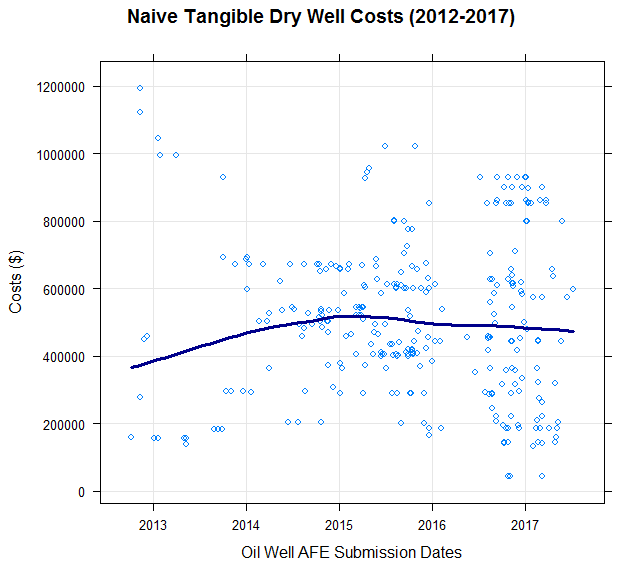
\includegraphics[width=.8\linewidth]{NaiveTangibleDry}
  \label{fig:sub1}
\end{subfigure}%
\begin{subfigure}{.5\textwidth}
  \centering
  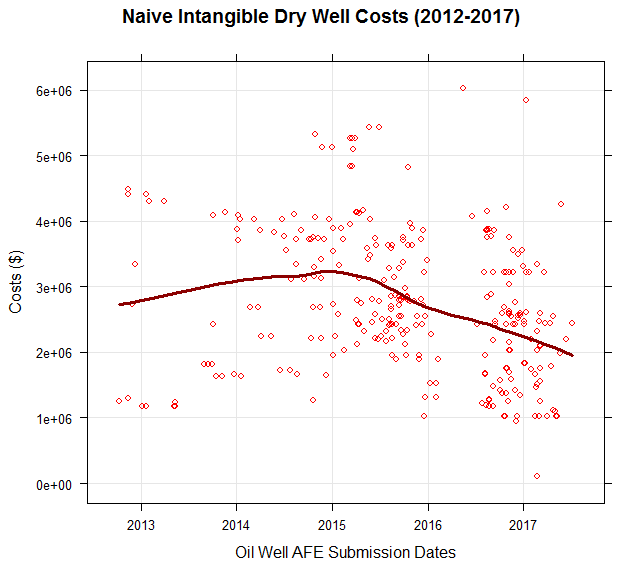
\includegraphics[width=.8\linewidth]{NaiveIntangibleDry}
  \label{fig:sub2}
\end{subfigure}
\label{fig:test}
\end{figure}
\\\\
\begin{figure}[h]
\centering
\begin{subfigure}{.5\textwidth}
  \centering
  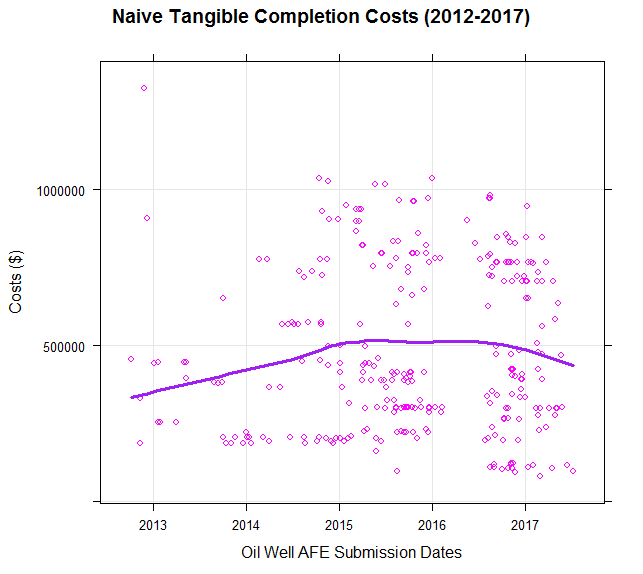
\includegraphics[width=.8\linewidth]{NaiveTangibleCompletion}
  \label{fig:sub1}
\end{subfigure}%
\begin{subfigure}{.5\textwidth}
  \centering
  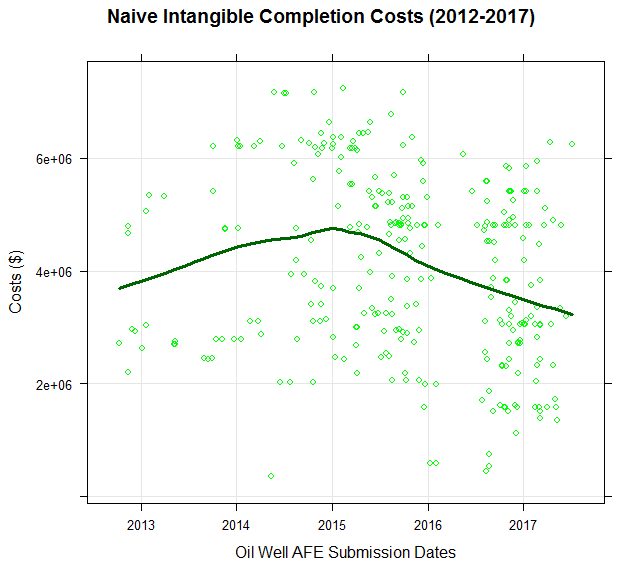
\includegraphics[width=.8\linewidth]{NaiveIntangibleCompletion}
  \label{fig:sub2}
\end{subfigure}
\caption{Naive local regressions of oil well cost data from 2012-2017, Oklahoma}
\label{fig:test}
\end{figure}
\\\\\\\\\\\\\\\\\\\\
\break
\\\\\\\\\\\\\\\\
\section{Length-Adjusted LOESS Analysis of Oil Well Costs Over Time 2012-17}
\\
\begin{figure}[h]
\centering
\begin{subfigure}{.5\textwidth}
  \centering
  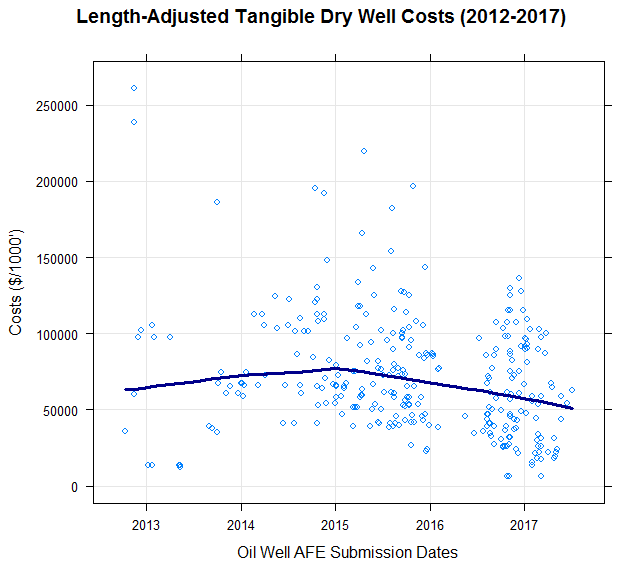
\includegraphics[width=.8\linewidth]{LengthTangibleDryWell}
  \label{fig:sub1}
\end{subfigure}%
\begin{subfigure}{.5\textwidth}
  \centering
  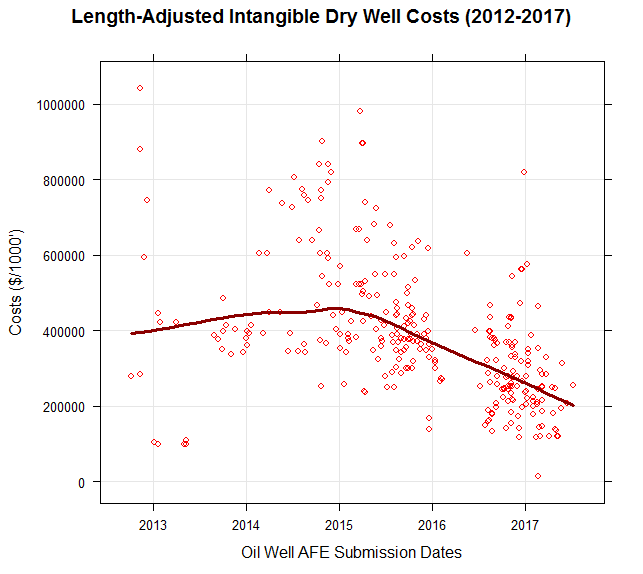
\includegraphics[width=.8\linewidth]{LengthIntangibleDryWell}
  \label{fig:sub2}
\end{subfigure}
\label{fig:test}
\end{figure}
\\\\
\begin{figure}[h]
\centering
\begin{subfigure}{.5\textwidth}
  \centering
  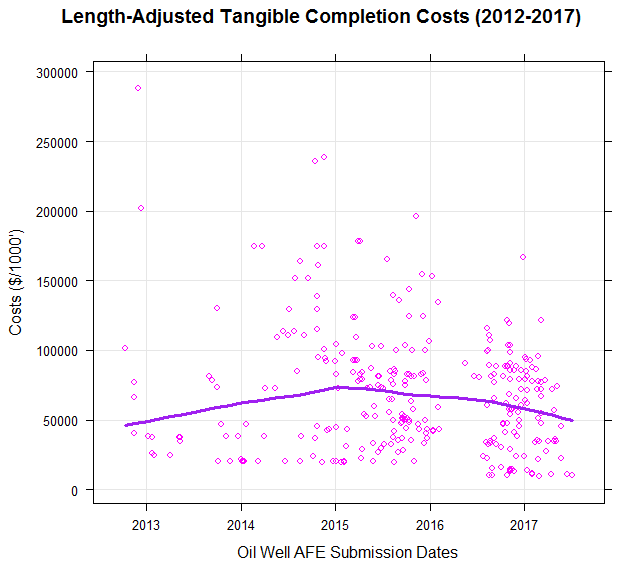
\includegraphics[width=.8\linewidth]{LengthTangibleComp}
  \label{fig:sub1}
\end{subfigure}%
\begin{subfigure}{.5\textwidth}
  \centering
  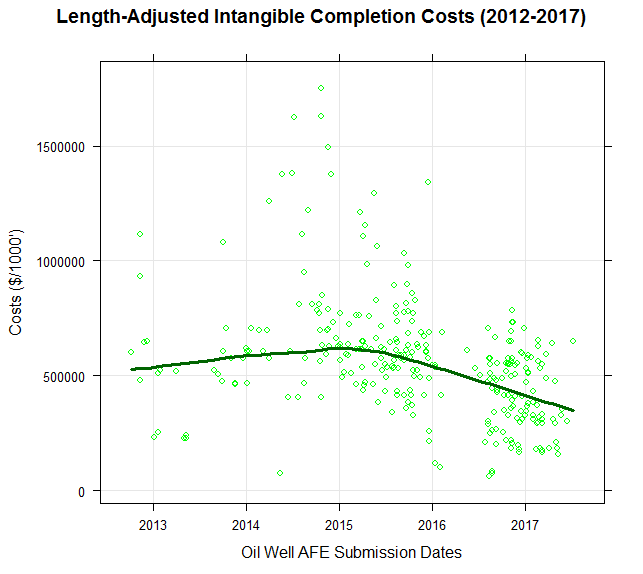
\includegraphics[width=.8\linewidth]{LengthIntangibleComp}
  \label{fig:sub2}
\end{subfigure}
\caption{Length-adjusted (per 1000') local regressions of oil well costs from 2012-2017, Oklahoma}
\label{fig:test}
\end{figure}
\\\\
\includegraphics[scale=0.35]{testing3}
\\\\
\includegraphics[scale=0.35]{testing4}
\\\\
\includegraphics[scale=0.35]{testing5}
\\\\
\includegraphics[scale=0.35]{testing6}
\\\\
\end{enumerate}
\end{document}